\PassOptionsToPackage{usenames,dvipsnames}{xcolor}
\documentclass[modern]{descnote}
\pdfoutput=1 %for arXiv submission
\usepackage[T1]{fontenc}
\usepackage{ae,aecompl}
\usepackage[utf8]{inputenc}
\usepackage{newtxtext,newtxmath}
\usepackage[english]{babel}
\usepackage{amsmath,amstext}
\usepackage[figure,figure*]{hypcap}
\usepackage{threeparttablex}
\usepackage{longtable}
\usepackage{inconsolata}

\definecolor{DESCred}{rgb}{0.63,0.00,0.20}
\hypersetup{colorlinks=true,breaklinks=true,
  citecolor=DESCred,filecolor=DESCred,linkcolor=DESCred,urlcolor=DESCred}

%figure pathhttps://www.overleaf.com/project/5fc85a437ab1bf2161bc7294
\graphicspath{{figs/}}

% for \autoref
\renewcommand*\sectionautorefname{Section}
\renewcommand*\subsectionautorefname{Section}
\renewcommand*\subsubsectionautorefname{Section}

%%%%% Custom commands %%%%%%

% For creating hyperlinks
\newcommand*{\https}[1]{\href{https://#1}{\nolinkurl{#1}}}
\newcommand*{\http}[1]{\href{http://#1}{\nolinkurl{#1}}}

% Other useful commands
\DeclareUrlCommand\code{\urlstyle{tt}}

% Commands for editing and revisions
\newcommand{\todo}[1]{\textcolor{orange}{#1}}


%%%%% Front Matter %%%%%%

\shorttitle{DESC DC2 Data Release Note}
\shortauthors{LSST~DESC}

\begin{document}
\title{DESC DC2 Data Release Note}
\collaboration{1000}{The LSST Dark Energy Science Collaboration (LSST DESC)}
\noaffiliation

\author{\textbf{(Incomplete Author List)}}
\noaffiliation

\author[0000-0002-1345-1359]{Joanne R. Bogart}
\affiliation{SLAC National Accelerator Laboratory, Menlo Park, CA 94025, USA}
\affiliation{Kavli Institute for Particle Astrophysics and Cosmology, Stanford University, Stanford, CA  94305, USA}

\author[0000-0001-5738-8956]{James Chiang}
\affiliation{SLAC National Accelerator Laboratory, Menlo Park, CA 94025, USA}
\affiliation{Kavli Institute for Particle Astrophysics and Cosmology, Stanford University, Stanford, CA  94305, USA}

\author[0000-0003-1468-8232]{Katrin~Heitmann}
\affiliation{Argonne National Laboratory, Lemont, IL 60439, USA}

\author[0000-0002-4394-6192]{Heather M. Kelly}
\affiliation{SLAC National Accelerator Laboratory, Menlo Park, CA 94025, USA}
\affiliation{Kavli Institute for Particle Astrophysics and Cosmology, Stanford University, Stanford, CA  94305, USA}

\author[0000-0002-2545-1989]{Eve Kovacs}
\affiliation{Argonne National Laboratory, Lemont, IL 60439, USA}

\author[0000-0003-2271-1527]{Rachel Mandelbaum}
\affiliation{McWilliams Center for Cosmology, Department of Physics, Carnegie Mellon University, Pittsburgh, PA 15213, USA}

\author[0000-0002-1200-0820]{Yao-Yuan~Mao}
\altaffiliation{NASA Einstein Fellow}
\affiliation{Department of Physics and Astronomy, Rutgers, The State University of New Jersey, Piscataway, NJ 08854, USA}

\author[0000-0003-3136-9532]{F. Javier S\'{a}nchez}
\affiliation{Department of Physics and Astronomy, University of California, Irvine, Irvine, CA 92697, USA}
\affiliation{Fermi National Accelerator Laboratory, PO Box 500, Batavia, IL 60510, USA}

\author[0000-0003-2035-2380]{Christopher W. Walter}
\affiliation{Department of Physics, Duke University, Durham NC 27708, USA }

\author[0000-0001-7113-1233]{W. Michael Wood-Vasey}
\affiliation{Department of Physics and Astronomy, University of Pittsburgh, Pittsburgh, PA 15260, USA}
\affiliation{Pittsburgh Particle Physics, Astrophysics and Cosmology Center (PITT PACC), University of Pittsburgh, Pittsburgh, PA 15260, USA}


\begin{abstract}
%\clearpage
%
Abstract text
%
\clearpage
\end{abstract}

\tableofcontents

\clearpage

\section{Introduction}

In the next decade, an unprecedented survey of the sky will be carried out using the Vera C. Rubin Observatory, the Legacy Survey of Space and Time \citep{2009arXiv0912.0201L,2019ApJ...873..111I}. One of the major aims of the survey is to unravel the origin of the cause of the accelerated expansion of the Universe. The LSST Dark Energy Science Collaboration (DESC)\footnote{\url{https://lsstdesc.org/}} was formed to carry out this exciting endeavor~\citep{Abate:2012za}. In order to prepare for the arrival of data, LSST DESC has generated two data challenges, DC1 and DC2, using sophisticated cosmological and  image simulations. %The data challenges have been designed to mimic actual data from the Rubin Observatory as closely as possible. As such, they cover a small, representative area of the planned LSST observing footprint.
The data challenges have been designed to mimic actual data from the Rubin Observatory in a small, representative area of the LSST observing footprint.
%The data challenges have been designed to provide LSST-like data to the collaboration

Both LSST DESC data challenges are based on realistic simulations of the extragalactic sky and employ a comprehensive image simulation library with a range of features, imSim. The resulting synthetic data were processed with Rubin's LSST Science Pipelines~\citep{2017ASPC..512..279J} to generate the final data products. The first data challenge, DC1, covers a $\sim$40 deg$^2$ area and ten years of observations. The image simulations were carried out for $r$-band only. A detailed description and a range of analysis results are provided in~\cite{dc1}.  In this data release note, we focus on the second data challenge, DC2. A comprehensive description of the LSST DESC DC2 Simulated Sky Survey can be found in~\cite{2020arXiv201005926L}. DC2 covers $\sim$300 deg$^2$ in the wide-fast-deep (WFD) area to be surveyed by LSST. Within this area, a small 1~deg$^2$ deep-drilling field (DDF) has been simulated as well. For the data release described in this note, only data from the WFD campaign and 5 years of observations are provided, corresponding to the planned sixth Rubin data release, DR6. For DC2, all six optical bands $ugrizy$ are included in the image simulations. The simulations, both for the extragalactic catalog and image generation, have many features that are relevant and realistic. However, given the complexity of the actual data and finite resources available, some features are less realistic or simply omitted. \cite{2020arXiv201005926L} provide a comprehensive discussion about the DC2 design choices that have been guided mostly by considerations regarding cosmological probes.  

For LSST DESC, the data challenges serve multiple purposes. The advantage of simulated data is that the underlying truth is known. Therefore, even if they are not as complex as observational data or have different systematics, they provide an excellent testbed for DESC analysis pipelines. Given that the data formats closely mimic the Rubin data products, they also serve to aid the development and optimization of data access methods. The data challenges also offer the opportunity to exercise the LSST Science Pipelines and investigate their performance, in particular with regard to how systematic effects in the data are handled. By making a first set of the data products publicly available, we hope that other LSST Science Collaborations will be able to carry out useful tests as part of preparations for data arrival preparation as well. In addition, the data should be of value for the broader optical astronomy and cosmology community.

This note is organized as follows. In~\autoref{sec:features} we describe the major features of the DC2 data set. We provide an overview of the data products that are part of this release in~\autoref{sec:products}. We provide instructions for data access, including a set of example Python Jupyter notebooks, in~\autoref{sec:access}.
%Together with the data itself, we release a set of selected notebooks that contain examples for common data analysis tasks. The notebooks are introduced in~\autoref{sec:notebooks}.
%In Section~\autoref{sec:validation} we present our validation and characterization of the DC2 data products.
We conclude in~\autoref{sec:outlook} and provide a brief description of possible future data releases. 

\section{Major Features of the Data Set}
\label{sec:features}

\subsection{Astrophysics Inputs}

The astrophysical components of this data set are mostly limited to the types of objects needed to support static probes of dark energy science, specifically the galaxies from the cosmoDC2 extragalactic catalog \citep{korytov}.  In addition, this data set includes stars from a simulated Milky Way, which are needed for the astrometric and photometric calibration by the image processing pipeline, as well as Type Ia supernovae, which were included throughout the 300~deg$^2$ DC2 region.

As noted, the galaxies are from the cosmoDC2 extragalactic catalog\footnote{Publicly available at \https{portal.nersc.gov/project/lsst/cosmoDC2/}}, which covers 440 deg$^2$ out to a redshift of $z = 3$ and is complete to $m_r <28$.  The cosmoDC2 catalog is based on the Outer Rim $N$-body simulation \citep{2019ApJS..245...16H}, and the properties of the galaxies were derived using the Galacticus semi-analytic model \citep{benson_2010b} and painted onto dark matter halos using GalSampler \citep{2020MNRAS.495.5040H}.  The derived galaxy properties include stellar mass, morphology, spectral energy distributions, broadband filter magnitudes, host halo information, and weak lensing shears.   The bulge and disk components of the galaxies are rendered separately as S\'ersic profiles, and galaxies with $m_i > 27$ have ``knots'' of star formation added in order to model more complex light profiles for the fainter galaxies. The fluxes for these star-forming regions have been re-allocated from the disk component, and the knots have the same spectral energy distribution (SED) as the disk.

The Milky Way stars are simulated using the Galfast model of \citet{2008ApJ...673..864J}, which is based on densities and colors of sources in the SDSS. Stellar variability is included for periodic objects (e.g., RR Lyrae and Cepheids) and for non-periodic variables (e.g., CVs, flaring M-dwarfs, etc.).  Stars without a definitive variability class are modeled based on the Kepler Q17 data release \citep{2016ksci.rept....3T}.  The Galactic reddening is based on the three-dimensional model of \cite{2005AJ....130..659A}.

Finally, Type Ia supernovae have been added throughout the DC2 region out to a redshift of $z=1.4$ with a population density that is consistent with observations.

\subsection{Image Simulation Features}

DC2 used the \code{minion_1016} observing cadence\footnote{Publicly available at \https{docushare.lsst.org/docushare/dsweb/View/Collection-4604}}, which was the Rubin Observatory LSST baseline cadence at start of the DC2 simulations. This cadence provides the nominal field positions, telescope rotations, and filter selections for each 30-second pointing, as well as predicted seeing, airmass, and sky background components.  We have added random translational and rotational dithering to the nominal pointings in order to make the sky coverage more uniform.

The imSim simulation software uses the GalSim package \citep{2015A&C....10..121R} to render the astrophysical objects and the night sky.  The point-spread functions (PSFs) for each exposure are computed using a set of atmospheric phase screens that are realizations of Gaussian random fields with a Von Karman power spectrum.  In addition, the PSF calculation includes an optical model of the telescope based on modeling of the active optics system for Rubin Observatory.  After convolution with the PSF, objects are rendered on the LSST CCDs taking into account the instrumental throughput in each band, the object's SED shape within the bandpass, atmospheric effects such as differential chromatic refraction, and the convergence of the incident beam from the telescope optics. GalSim's sensor model includes the brighter-fatter and tree-ring electrostatic effects that are present in the CCDs used in the LSST Camera (LSSTCam).  Finally, electronics readout effects such as bleed trails, CCD segmentation, intra-CCD cross-talk, read noise, etc., are applied.  These effects are based on measurements of the actual LSSTCam hardware.


\section{Available Data Sets}
\label{sec:products}

This Data Release (v1) provides the data from the WFD campaign for 5 years of observations (corresponding to Rubin's DR6). This data set includes two ``Tables'': the ``Object Table'' and the ``Truth-match Table.'' We define these tables and describe their data models in the subsections below. 

\subsection{Object Table}
\label{sec:object}

The Object Table contains information about static astronomical objects measured on a stacked (coadd) image. The photometry in the Object Table is measured with the forced photometry method, i.e., it is consistently measured across multiple bands using a fixed position, which is determined from the reference band for each source \citep[Sec.~3.4 of][]{10.1093/pasj/psx080}. 

The generation of the Object Table is described in detail in \S~8 of \cite{2020arXiv201005926L}. In short, after the LSST Science Pipelines (v19) produce the deepCoadd catalogs of multiple bands, we merge these catalogs across bands, and apply certain column renaming and translations to produce the final Object Table. The renaming and translations are meant to produce a science-ready catalog that resembles the Rubin LSST Data Products Definition Document (LSE-163; \https{lse-163.lsst.io}) for the end users. 

Each entry (row) in the Object Table corresponds to one measured astronomical object, assigned with a unique ID (\code{objectID}). There are no duplicated entries in the Object Table. For details about the physical representation of the Object Table, see \autoref{sec:representation}. The full schema for the Object Table can be found in \autoref{app:object-schema}. 

\subsection{Truth-match Table}
\label{sec:truth}

The Truth-match Table is a joint representation of both the truth information (i.e., the measurable fluxes and positions of astronomical objects that serve as input values to the image simulations) and their best matches to the measured objects in the Object Table. The Truth-match Table allows users to examine, for example, the differences between true and measured fluxes and positions, and compare to the expected levels of photometric and astrometric accuracy and precision.

The generation of the Truth-match Table is described in \S\,4.2.1 of \cite{2020arXiv201005926L}. The truth information in the Truth-match Table only includes ``summary'' properties (i.e., static, or infinite-time averaged fluxes) of galaxies (including infinite-time averaged AGN components \todo{check with Joanne}), stars, and supernovae (SNe). Time-varying properties are not included. The match information stored in the  Truth-match Table is produced with the following procedure applied for each entry in the Object Table:
\begin{enumerate}
    \item Search for all truth entries that are within 1~arcsec and have a $r$-band magnitude difference ($\Delta r$) less than 1~mag. If one or more truth entries that satisfy these criteria are found, pick the truth entry that has the smallest $|\Delta r|$ as the match, and set \code{is_good_match} to True.
    \item If no truth entry was found in Step (1), pick the truth entry that is the nearest neighbor of the object entry on sky as the match, and set \code{is_good_match} to False.
\end{enumerate}
Given this procedure, every entry in the Object Table is assigned exactly one match. The majority of object entries have a ``good'' match (i.e., satisfying criteria in Step 1 above), and the rest have a nearest-neighbor match. More than 90\% of the ``good'' matches are not only the closest match in magnitude, but also the nearest neighbor match. 

Because the Object Table was used as the reference catalog for the matching procedure, some truth entries may be chosen as a match more than once, while others may not be chosen as a match at all.
Flags to distinguish these situations are included in the Truth-match Table. 
Selecting all entries with \code{match_objectId} $> -1$ from the Truth-match Table would result in a subset of Truth-match entries that have exactly the same row order as the entries in the Object Table (and hence may contain duplicated truth entries). On the other hand, selecting all entries with \code{is_unique_truth_entry} being True would produce a subset of Truth-match entries that contain all unique truth entries, including truth entries that have not been chosen as a match.
These selections are particularly important for users who wish to access the files directly. For users who use GCRCatalogs (\autoref{sec:gcr}), the reader will automatically select the correct rows depending on whether you are loading the Truth Table or the Match Table (see \autoref{sec:notebooks} for examples).

The physical representation of the Truth-match Table is described in \autoref{sec:representation}. The full schema for the Truth-match Table can be found in \autoref{app:truth-schema}.



\section{Data Access}
\label{sec:access}


\subsection{Physical Representation of the Data Sets}
\label{sec:representation}

All data tables in this release are stored in the Apache Parquet\footnote{\https{parquet.apache.org}} format, an efficient columnar storage form, with I/O tools readily available for multiple development systems. 
The data files can be easily downloaded to the user's machine via Globus (\autoref{sec:download}), and read with Python packages such as \code{pyarrow} or \code{fastparquet}.
We additionally provide a Python package, \code{GCRCatalogs}, which contains a high-level user API to access the data files (\autoref{sec:gcr}). 

Each data table is further partitioned into several files that correspond to different parts of the sky. The partition is based on the ``tract'' value in the ``Rings sky map'' pixelization of LSST Science Pipelines.\footnote{\https{pipelines.lsst.io/py-api/lsst.skymap.ringsSkyMap.RingsSkyMap.html}} \autoref{fig:skymap} shows a visual representation of the partition. The same partition is used for both Object Table and Truth-match Table. No padding is included; i.e., an entry that is near the tract boundary still only appears in the tract it belongs to. Each Parquet file contains only one partition (row group). 

\begin{figure}[tbh!]
    \centering
    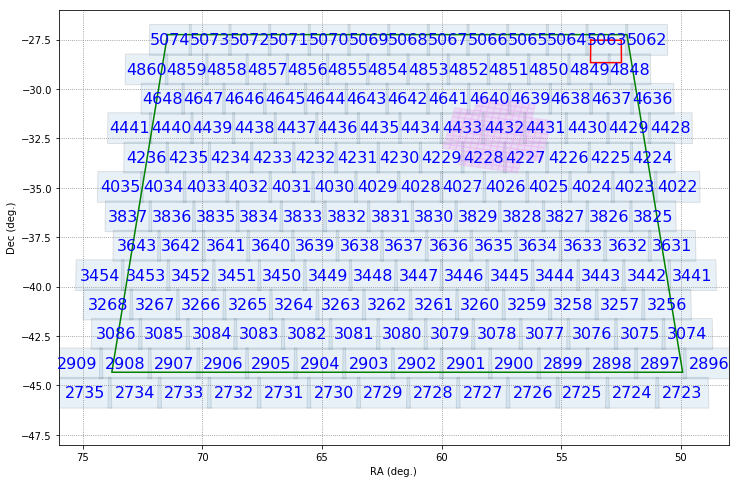
\includegraphics[width=0.8\textwidth]{figs/skymap.png}
    \caption{Sky Map}
    \label{fig:skymap}
\end{figure}



\subsection{Downloading Data Files}
\label{sec:download}

\subsection{Accessing Data in Python}
\label{sec:gcr}


\subsection{Example Python Jupyter Notebook}
\label{sec:notebooks}

We provide two example Python Jupyter Notebooks to demonstrate how to use \code{GCRCatalogs} to access the data, explain the data model, and show a few simple analyses that can be used as starting points for further development. 
These Jupyter Notebooks can be found in the associated GitHub repository.\footnote{\url{https://github.com/LSSTDESC/DC2-Public-Release}}

\section{Conclusion and Outlook}
\label{sec:outlook}

In this note we described the first public data release for DC2 carried out by the LSST DESC. We make data available for a simulated WFD survey spanning 300 degree$^2$ and 5 years of Rubin observations, including a subset of the coadd-based catalogs that would be included in Rubin Observatory's DR6. We provided a brief overview of the major features of the data set in~\autoref{sec:features} and a detailed description of the available products in~\autoref{sec:products}. The data can be accessed via a web-portal that offers a convenient interface for data transfers using Globus as described in~\autoref{sec:access}. In order to enable first quick experiments, we also release a set of example notebooks, as described in~\autoref{sec:notebooks}. We encourage new users to provide feedback and ask questions via a dedicated GitHub repository.\footnote{\url{https://github.com/LSSTDESC/DC2-Public-Release}}

This Data Release (v1) focuses on a limited set of data products generated with the LSST Science Pipelines. In the future, we plan to extend this data release in several directions. First, LSST DESC is currently working on generating so-called ``add-on'' catalogs. These catalogs provide additional information obtained from further processing the data. Examples include a photo-z catalog and a cluster catalog. Once these catalogs have been carefully validated and are of sufficient quality to be of broader interest, they will be added to the DC2 Data Release. Second, the processing of the DDF portion of DC2 is still in progress. As explained in more detail in~\cite{2020arXiv201005926L}, the DDF region contains several astrophysical components, e.g.~AGNs, that are not available in the WFD region. As with the add-on catalogs, once careful validation has concluded, we plan to make those data available as well. Finally, for cosmology it is very informative to compare results from different data releases to build a better understanding of the impact of the depth of the data on cosmological constraints. Therefore, LSST DESC is currently generating additional coadds and associated catalogs for subsets of the data corresponding to 1- and 2-year depth. Depending on the feedback we receive, these datasets will become part of future public data releases as well.


%%%%%% Appendices %%%%%% 
\clearpage
\appendix
\section{Changelog}
\begin{ThreePartTable}
\begin{TableNotes}
\footnotesize
\item[] ~
\end{TableNotes}
\begin{widetext}
\begin{longtable}{p{0.8in}p{0.8in}p{4in}}
\hline
\textbf{Date} & \textbf{Version} & \textbf{Description} \\ 
\hline
\endhead
\endfoot
\hline
\insertTableNotes  % tell LaTeX where to insert the contents of "TableNotes"
\endlastfoot
06/16/2025 & v5 & The center coordinates of the WFD region stated in \autoref{sec:features:astro} are corrected. \\
06/15/2022 & v4 & (1) New data sets available in this release: (a) unmerged truth catalogs (summaries for SNe, stars and galaxies and variability information for stars and SNe; \autoref{sec:truth-unmerged}), and (b) additional intermediate data products (calibrated exposures, background subtracted images, and source catalogs output from the single-epoch processing;  \autoref{sec:intermediate-data-products}). (2) Truth table and Truth-match table have been updated to match the unmerged truth catalogs. (3) ``Known Issues'' section was added to this note. \\
12/10/2021 & v3 & The URL to DESC Data Portal was updated. \\
06/08/2021 & v2 & A minor processing issue was fixed in Tract 4852; the object and truth-match tables are updated. Two tracts of coadded images are provided. \\
01/07/2021 & v1 & Initial release \\
\end{longtable}
\end{widetext}
\end{ThreePartTable}

\clearpage

\section{Table Schema}

\subsection{Object Table Schema}
\label{app:object-schema}
\begin{ThreePartTable}
\begin{TableNotes}
\footnotesize
\item [\hypertarget{obj_fn1}{1}] In LSE-163, \code{I<xx,yy,xy>} and \code{I<xx,yy,xy>PSF} are defined in the units of squared arcsec. 
\end{TableNotes}
\begin{longtable}{p{1.7in}p{0.5in}p{0.6in}p{2.8in}}
\hline
\textbf{Name} & \textbf{Type} & \textbf{Unit} & \textbf{Description} \\ 
\hline
\endhead
\endfoot
\hline
\insertTableNotes  % tell LaTeX where to insert the contents of "TableNotes"
\endlastfoot
\code{objectId} & int64 & -- & Unique object ID \\
\code{parentObjectId} & int64 & -- & Parent object ID \\
%
\code{good} & bool & -- & True if the source has no flagged pixels \\
\code{clean} & bool & -- &  True if the source has no flagged pixels (i.e., \code{good}) and is not skipped by the deblender \\
\code{blendedness} & float64 & -- & Measure of how flux is affected by neighbors ($1 - I_\text{child}/I_\text{parent}$; see \S\,4.9.11 of \citealt{10.1093/pasj/psx080}) \\
\code{extendedness} & float64 & -- & 0 for stars; 1 for extended objects \\
\code{ra} & float64 & degree & Right Ascension \\
\code{dec} & float64 & degree & Declination \\
\code{x} & float64 & pixel & 2D centroid location (x coordinate) \\
\code{y} & float64 & pixel & 2D centroid location (y coordinate) \\
\code{xErr} & float32 & pixel & Error value for \code{x} \\
\code{yErr} & float32 & pixel & Error value for \code{y} \\
\code{xy_flag} & bool & -- & Flag for issues with \code{x} and \code{y} \\
\code{tract} & int64 & -- & Tract ID in Sky Map \\ 
\code{patch} & string & -- & Patch ID in Sky Map (as a string, \code{`x,y'})\\ 
%
\code{Ixx_pixel} & float64 & sq.~pixel$^\text{\hyperlink{obj_fn1}{1}}$ & Adaptive second moment ($xx$) of source intensity, averaged across bands \\
\code{Ixx_pixel_<band>} & float64 & sq.~pixel$^\text{\hyperlink{obj_fn1}{1}}$ & Adaptive second moment ($xx$) of source intensity in \code{<band>} \\
\code{Iyy_pixel} & float64 & sq.~pixel$^\text{\hyperlink{obj_fn1}{1}}$ & Adaptive second moment ($yy$) of source intensity, averaged across bands \\
\code{Iyy_pixel_<band>} & float64 & sq.~pixel$^\text{\hyperlink{obj_fn1}{1}}$ & Adaptive second moment ($yy$) of source intensity in \code{<band>} \\
\code{Ixy_pixel} & float64 & sq.~pixel$^\text{\hyperlink{obj_fn1}{1}}$ & Adaptive second moment ($xy$) of source intensity, averaged across bands \\
\code{Ixy_pixel_<band>} & float64 & sq.~pixel$^\text{\hyperlink{obj_fn1}{1}}$ & Adaptive second moment ($xy$) of source intensity in \code{<band>} \\
\code{I_flag} & bool & -- & Flag for issues with \code{Ixx}, \code{Iyy_pixel}, and \code{Ixy} \\
\code{I_flag_<band>} & bool & -- & Flag for issues with \code{Iyy_pixel_<band>}, \code{Ixy_<band>}, and \code{Ixx_<band>} \\
\code{IxxPSF_pixel} & float64 & sq.~pixel$^\text{\hyperlink{obj_fn1}{1}}$ & Adaptive second moment ($xx$) of PSFy, averaged across bands \\
\code{IxxPSF_pixel_<band>} & float64 & sq.~pixel$^\text{\hyperlink{obj_fn1}{1}}$ & Adaptive second moment ($xx$) of PSF in \code{<band>} \\
\code{IyyPSF_pixel} & float64 & sq.~pixel$^\text{\hyperlink{obj_fn1}{1}}$ & Adaptive second moment ($yy$) of PSFy, averaged across bands \\
\code{IyyPSF_pixel_<band>} & float64 & sq.~pixel$^\text{\hyperlink{obj_fn1}{1}}$ & Adaptive second moment ($yy$) of PSF in \code{<band>} \\
\code{IxyPSF_pixel} & float64 & sq.~pixel$^\text{\hyperlink{obj_fn1}{1}}$ & Adaptive second moment ($xy$) of PSFy, averaged across bands \\
\code{IxyPSF_pixel_<band>} & float64 & sq.~pixel$^\text{\hyperlink{obj_fn1}{1}}$ & Adaptive second moment ($xy$) of PSF in \code{<band>} \\
\code{psf_fwhm_<band>} & float64 & arcsec & PSF FWHM calculated from \code{base_SdssShape} \\
\code{psNdata} & float32 & - & Number of data points (pixels)
used to fit the model \\
%
\code{psFlux_<band>} & float64 & nJy & Point-source model flux in \code{<band>} \\
\code{psFluxErr_<band>} & float64 & nJy & Error value for \code{psFlux_<band>} \\
\code{psFlux_flag_<band>} & bool & -- & Flag for issues with \code{psFlux_<band>} \\
\code{mag_<band>} & float64 & AB mag & Point-source model magnitude in \code{<band>}\\
\code{magerr_<band>} & float64 & AB mag & Error value for \code{mag_<band>} \\
%
\code{cModelFlux_<band>} & float64 & nJy & Composite model (cModel) flux in \code{<band>} \\
\code{cModelFluxErr_<band>} & float64 & nJy & Error value for \code{cModelFlux_<band>} \\
\code{cModelFlux_flag_<band>} & bool & -- & Flag for issues with \code{cModelFlux_<band>} \\
\code{mag_<band>_cModel} & float64 & AB mag & cModel magnitude in \code{<band>} \\
\code{magerr_<band>_cModel} & float64 & AB mag & Error value for \code{mag_<band>_cModel} \\
\code{snr_<band>_cModel} & float64 & -- & Signal-to-noise ratio for cModel magnitude in \code{<band>} \\
\end{longtable}
\end{ThreePartTable}

\bigskip

\subsection{Truth-match Table Schema}
\label{app:truth-schema}
\begin{ThreePartTable}
\begin{TableNotes}
\footnotesize
\item [\hypertarget{truth_fn1}{1}] When accessing this catalog as \code{dc2_object_run2.2i_dr6_wfd_with_truth_match} via \code{GCRCatalogs}, all the columns in this table, except for the last six, are postfixed with \code{_truth}.
\item [\hypertarget{truth_fn2}{2}] Only present when accessing the catalog via \code{GCRCatalogs}.
\item [\hypertarget{truth_fn3}{3}] Because the object catalog is used as the reference catalog for matching, some truth entries may appear more than once, and some truth entries may not have a matching object.
\end{TableNotes}
\begin{longtable}{p{1.6in}p{0.5in}p{0.6in}p{2.9in}}
\hline
\textbf{Name}$^\text{\hyperlink{truth_fn1}{1}}$ & \textbf{Type} & \textbf{Unit} & \textbf{Description} \\ 
\hline
\endhead
\endfoot
\hline
\insertTableNotes  % tell LaTeX where to insert the contents of "TableNotes"
\endlastfoot
\code{id} & string & -- & Unique object ID \\ 
\code{host_galaxy} & int64 & -- & ID of the host galaxy for a SN entry ($-1$ for other truth types)\\ 
\code{ra} & float64 & degree & Right Ascension \\
\code{dec} & float64 & degree & Declination \\
\code{redshift} & float32 & -- & Redshift \\ 
\code{is_variable} & int32 & -- & 1 for a variable source \\ 
\code{is_pointsource} & int32 & -- & 1 for a point source \\ 
\code{flux_<band>} & float32 & nJy & Static flux value in \code{<band>} \\ 
\code{flux_<band>_noMW} & float32 & nJy & Static flux value in \code{<band>}, without Milky Way extinction (i.e., dereddened) \\ 
\code{mag_<band>}$^\text{\hyperlink{truth_fn2}{2}}$ & float32 & AB mag & Magnitude in \code{<band>} \\ 
\code{mag_<band>_noMW}$^\text{\hyperlink{truth_fn2}{2}}$ & float32 & AB mag & Magnitude in \code{<band>}, without Milky Way extinction (i.e., dereddened) \\ 
\code{tract} & int64 & -- & Tract ID in Sky Map \\ 
\code{patch} & string & -- & Patch ID in Sky Map (as a string, \code{`x,y'}) \\ 
\code{cosmodc2_hp} & int64 & -- & Healpix ID in cosmoDC2 (for galaxies only; $-1$ for stars and SNe) \\ 
\code{cosmodc2_id} & int64 & -- & Galaxy ID in cosmoDC2 (for galaxies only; $-1$ for stars and SNe)\\ 
\code{truth_type} & int64 & -- & 1 for galaxies, 2 for stars, and 3 for SNe \\ 
\code{match_objectId} & int64 & -- & \code{objectId} of the matching object entry ($-1$ for unmatched truth entries$^\text{\hyperlink{truth_fn3}{3}}$) \\ 
\code{match_sep} & float64 & arcsec & On-sky angular separation of this object--truth matching pair ($-1$ for unmatched truth entries$^\text{\hyperlink{truth_fn3}{3}}$) \\ 
\code{is_good_match} & bool & -- & \code{True} if this object--truth matching pair satisfies all matching criteria \\
\code{is_nearest_neighbor} & bool & -- & \code{True} if this truth entry is the nearest neighbor of the object specified by \code{match_objectId} \\
\code{is_unique_truth_entry} & bool & -- & \code{True} for truth entries that appear for the first time in this truth table$^\text{\hyperlink{truth_fn3}{3}}$ \\
\end{longtable}
\end{ThreePartTable}


%%%%%% Acknowledgments %%%%%% 
\clearpage
\section*{Acknowledgments}
\phantomsection
\addcontentsline{toc}{section}{Acknowledgements}

The DESC acknowledges ongoing support from the Institut National de 
Physique Nucl\'eaire et de Physique des Particules in France; the 
Science \& Technology Facilities Council in the United Kingdom; and the
Department of Energy, the National Science Foundation, and the LSST 
Corporation in the United States.  DESC uses resources of the IN2P3 
Computing Center (CC-IN2P3--Lyon/Villeurbanne - France) funded by the 
Centre National de la Recherche Scientifique; the National Energy 
Research Scientific Computing Center, a DOE Office of Science User 
Facility supported by the Office of Science of the U.S.\ Department of
Energy under Contract No.\ DE-AC02-05CH11231; STFC DiRAC HPC Facilities, 
funded by UK BIS National E-infrastructure capital grants; and the UK 
particle physics grid, supported by the GridPP Collaboration.  This 
work was performed in part under DOE Contract DE-AC02-76SF00515.


% Individual acknowledgments (sorted by author order)
The work of APH, KH, EK, PL, and ASV at Argonne National Laboratory was supported under the U.S. DOE contract DE-AC02-06CH11357.
Support for YYM was provided by NASA through the NASA Hubble Fellowship grant no.\ HST-HF2-51441.001 awarded by the Space Telescope Science Institute, which is operated by the Association of Universities for Research in Astronomy, Incorporated, under NASA contract NAS5-26555. 

% Contribution statements



%%%%%% References %%%%%% 
\clearpage
\phantomsection
\addcontentsline{toc}{section}{References}

\bibliographystyle{aasjournal}
\bibliography{ref}

\end{document}
